%%%%%%%%%%%%%%%%%%%%%%%%%%%%
\subsection{Ionization Laser System}
\label{sec:sp-calib-sys-las-ion}
%%%%%%%%%%%%%%%
%\subsubsection{Physics Motivation}
%\label{sec:sp-calib-sys-las-ion-phys} 
Through its effect on drift velocity, recombination and lifetime, the \efield is a critical parameter for physics signals as it ultimately impacts the spatial resolution and energy response of the detector. The primary purpose of a laser system is to provide an independent, fine-grained estimate of the \efield in space and time. 

Since it measures spatial distortions of straight tracks, the laser system actually measures the local drift velocity field directly and helps define the detector \dword{fv} and this in itself is an important input for the \dword{lbl} analysis. 
%, and this is in itself an input to the analysis.
%Still,
However, it is still important to use information independent from the charge in order to disentangle effects like lifetime and recombination from \efield distortions. The laser system can accomplish this, by using the position information to derive the \efield from the local velocity map, taking into account the colinearity between both vectors, and the relatively well studied relation on the magnitude (see~\cite{Li:2015rqa} and references [29, 45-58] therein). A laser system also has the intrinsic advantage of being immune to recombination, thus eliminating particle-dependent effects.  

There are multiple sources which may distort the \efield temporally  and/or spatially in the detector. Current simulation studies indicate that positive ion accumulation and drift (space charge) due to ionization sources such as cosmic rays or \Ar39 is small in the \dword{dune} \dword{fd}, causing \efield distortions of at most \SI{0.1}{\%}~\cite{bib:mooney2018}.
However, not enough is known yet about the fluid flow pattern in the \dword{fd} to exclude the possibility of stable eddies which may amplify the effect for both \single and \dual modules. This effect can get further amplified significantly in the \dword{dpmod} due to  accumulation in the liquid of ions created by the electron multiplication process in the gas phase.
%due to ion accumulation at the liquid-gas interface. 
Additionally, other sources in the detector (especially detector imperfections) can cause \efield distortions. For example, field cage resistor failures, non-uniform resistivity in the voltage dividers, \dword{cpa} misalignment, \dword{cpa} structural deformations, and \dword{apa} and \dword{cpa} offsets and  deviations from flatness can create localized \efield distortions. These effects are presented in Figures~\ref{fig:efield_cpa_distortions_boyu2017} and~\ref{fig:efield_resistorfailure_mooney2019}, that show the impact of a few \% on the \efield from \SI{2}{\cm} \dword{cpa} position tilts and of up to \SI{4}{\%} from field cage single resistor failures.

\begin{dunefigure}[Impact on \efield of CPA position distortions]{fig:efield_cpa_distortions_boyu2017}
{Illustration of a possible distortion of the \dword{cpa} position~\cite{bib:yu2017a}, assuming a \SI{2}{\cm} swing, and its impact on \efield (right).}
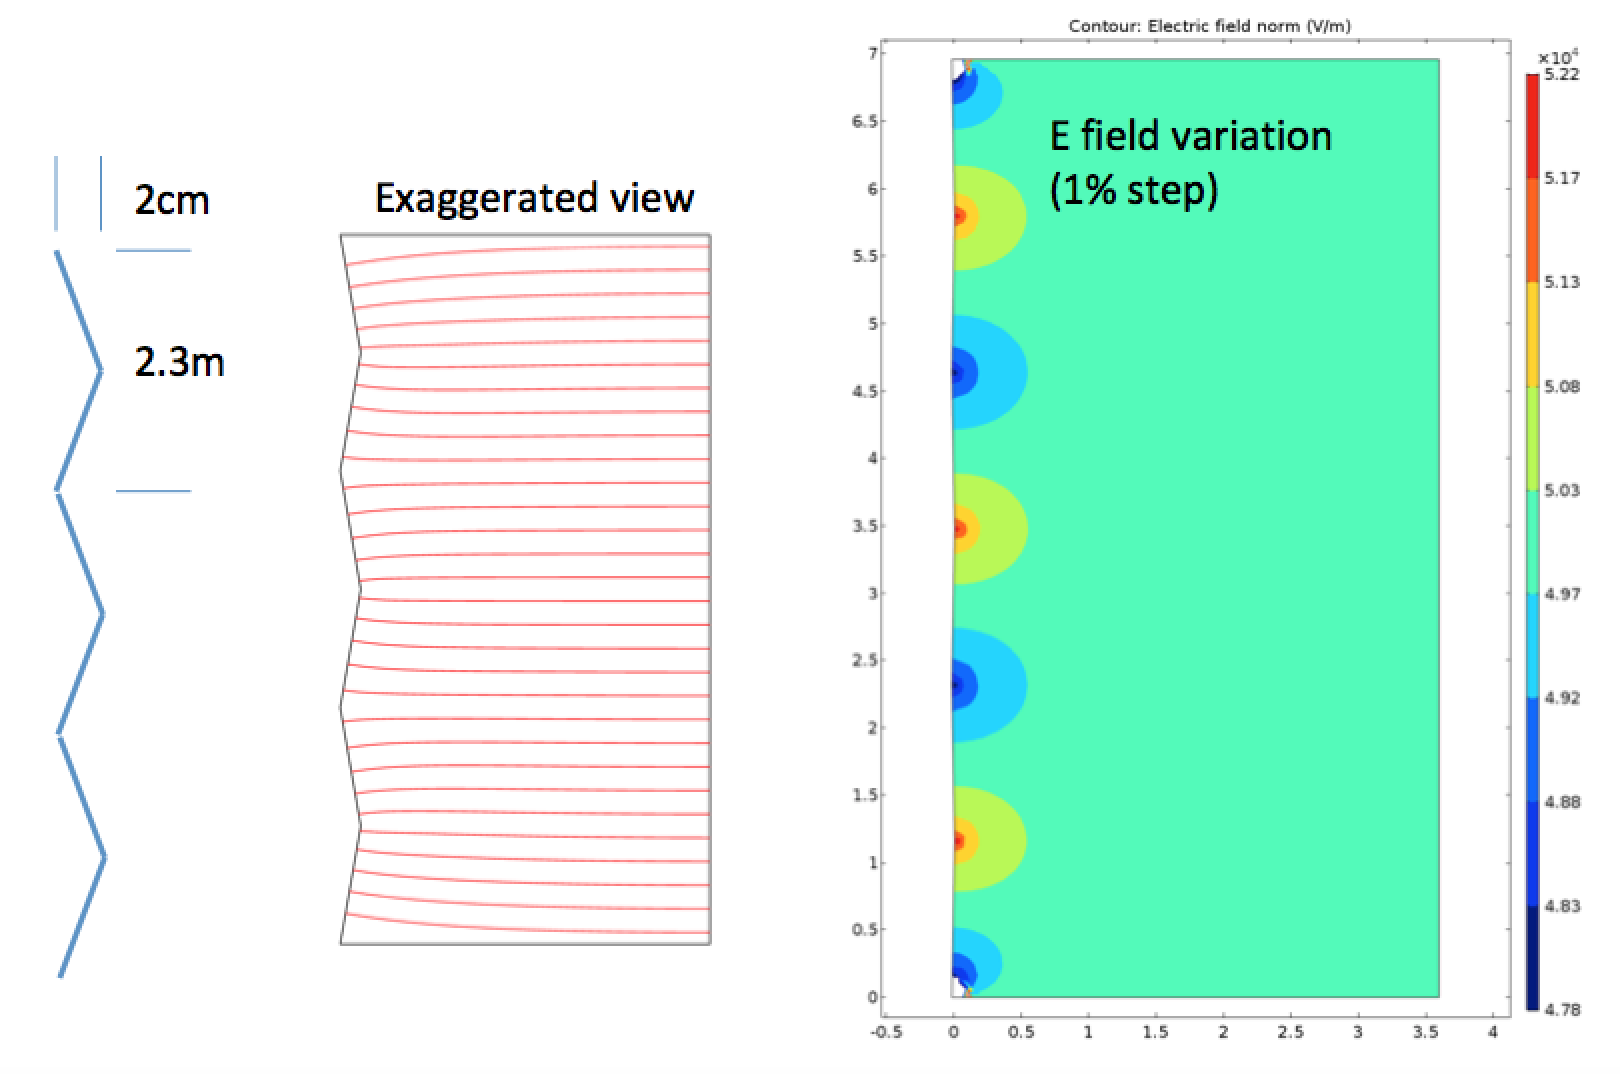
\includegraphics[width=0.8\textwidth]{efield_cpa_distortions_boyu2017.png}
\end{dunefigure}

\begin{dunefigure}[Impact on \efield of FC resistor failures]{fig:efield_resistorfailure_mooney2019}
{Impact on \efield magnitude distortions of a single \dword{fc} resistor failure~\cite{bib:mooney2019a}.}
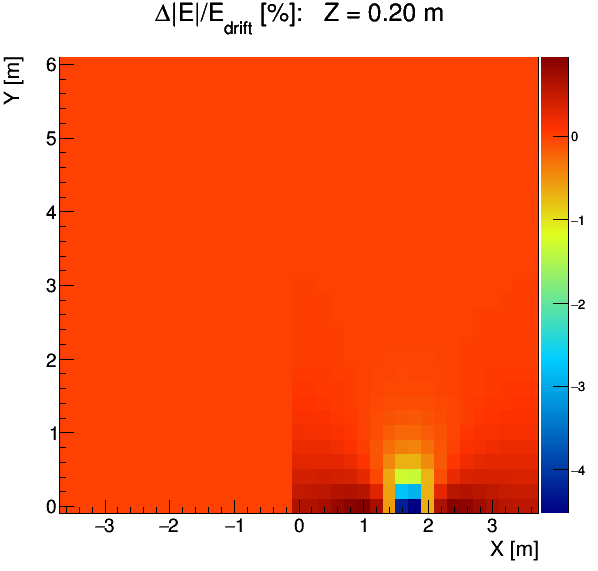
\includegraphics[width=0.5\textwidth]{efield_resistorfailure_mooney2019.png}
\end{dunefigure}

In both \single and \dual systems, the failure of a resistor will create significant, local electric field distortions which will need to be identified\footnote{In the \dual system, four resistors would have to fail to cause a failure across the field cage gap, but even one failure in the \dword{sp} can have an impact; this may be partially mitigated by modifying the HV, but not completely.}. While the resistor failure will be detected temporally, its location in space is not possible to determine from slow controls monitoring data. Misalignments of detector objects or deformations may also create (small) electric field distortions; while individual effects may be small, it is possible to have a combined, significant effect.
Each individual \efield distortion may add in quadrature with other effects, and can reach up to \SI{4}{\%} under certain conditions. Understanding all these effects requires in-situ measurement of \efield for proper calibration. 

Many useful secondary uses of laser include alignment (especially modes that are weakly constrained by cosmic rays),
%; see Figure~\ref{fig:apacurtainalign}),
stability monitoring, and diagnosing detector performance issues
%failures 
(e.g., \dword{hv}).  
Misalignment may include physical deformation and/or rotations of objects within the detector. Given the expected low rate of cosmic ray events (about 3500/day/10-kt) at the underground location, calibration with cosmic rays is not possible over short time scales. Certain alignment ``directions''  are difficult to assess with cosmic rays alone, such as distortions of the detector that preserve the gap widths and do not shift the \dwords{apa} in $x$ near the gaps relative to one another.
These distortions include global shifts and rotations in the locations of all detector elements, and crumpling modes where the edges of the \dwords{apa} hold together but angles are slightly different from nominal.   

%A laser system also has the intrinsic advantage of being immune to recombination, thus eliminating particle-dependent effects.  




%%%%%%%%%%%%%%%%%%%%%%%%%%%%
\subsubsection{Requirements}
\label{sec:sp-calib-laser-req}


%\fixme{SG, KM: Done; JM please check. }
%To-DO: Need more information on requirements from neutron source and RA source, once we have it, we can update the text/table as needed.}

Some common design considerations for calibration devices include stability, reliability, and longevity, so calibration systems can be operated for the lifetime of the experiment (\dunelifetime). Such longevity is uncommon for any device, so the overall design permits replacing devices where possible, namely the parts that are external to the cryostat. The systems must also adhere to relevant global requirements of the \dword{dune} detector. Table~\ref{tab:specs:SP-CALIB} shows the top-level overall requirements for calibration subsystems along with global \dword{dune} requirements that are relevant for calibration. For example, \dword{dune} requires the \efield  on any instrumentation devices inside the cryostat to be less than 30 kV/cm to minimize the risk of dielectric breakdown in \dword{lar}. Another consideration important for event reconstruction is understanding the maximum tolerable level of noise on the readout electronics due to calibration devices and implementing proper grounding schemes to minimize it. 
%Another consideration important for reconstructing events is the maximum noise level the readout electronics can tolerate from calibration devices \todo{Jose to check the next part of the sentence} and implementing proper grounding scheme to minimize noise issues. 
\dword{pdsp} is evaluating this. In Table~\ref{tab:specs:SP-CALIB}, two values are quoted for most of the parameters: 1) specification, which is the minimum requirement to guarantee baseline performance, and 2) goal, an ideal requirement %enabling more detailed studies and 
for achieving improved precision.

For the ionization laser system, the energy and position reconstruction requirements for physics measurements lead to requirements for the necessary precision in measuring the \dword{tpc} \efield as well as its spatial coverage and granularity. The precision of the \efield measurement with the laser system must be about \SI{1}{\%} so that the effect from \efield on the collected charge, via the dependence of the recombination factor on \efield, is well below \SI{1}{\%}. This is also motivated by consistency with the high level \dword{dune} specification of \SI{1}{\%} on field uniformity throughout the volume for component alignment and the \dword{hv} system. For laser coverage, to keep the \efield measurement at the $\sim$\SI{1}{\%} level, we are aiming for a coverage of \SI{75}{\%} or more of the total \dword{fv}. The requirement on granularity for the laser is estimated based on the \dword{fv} uncertainty requirements (\SI{1}{\%}) and corresponding uncertainty requirements (\SI{1.5}{\cm}) in each coordinate. A specification is set for a voxel size of \num{30}$\times$\num{30}$\times$\SI{30}{\cubic\cm}, that should be sufficient to satisfy the \dword{fv} uncertainty requirements. A goal is set for \num{10}$\times$\num{10}$\times$\SI{10}{\cubic\cm}, which could allow for a refinement in precision in some detector regions. 

The laser beam location must also meet the level of reconstruction requirement in each coordinate, approximately \SI{5}{\milli\m}. In order to reach that over distances of up \SI{20}{\m}, where the latter is the maximum distance that any beam needs to travel to cover all detector voxels, this results in a stringent requirement of \ang{0.015} (or \SI{0.25}{\mrad}) on the pointing precision. The laser beam location system is also designed to check the beam location with a precision of \SI{5}{\milli\m} over distances of up \SI{20}{\m}.
%\SI{5}{\milli\m} over \num{5} to \SI{10}{\m}, where the latter is the distance between two consecutive laser ports in the beam direction. This results in a stringent requirement of \ang{0.03} (or \SI{0.5}{\mrad}).
The data volume for the ionization laser system must be at least \num{184}~TB/year/\SI{10}{\kt}, assuming \num{800}k laser pulses, \num{10}$\times$\num{10}$\times$\SI{10}{\cubic\cm} voxel sizes, a \SI{100}{\micro\s} zero suppression window, and two dedicated calibration campaigns per year.

For the \dword{pns} system, the system must provide sufficient neutron event rate to make spatially separated precision measurements across the detector of a comparable size to the voxels probed by the laser (\num{30}$\times$\num{30}$\times$\SI{30}{\cubic\cm}) for most regions of the detector (\SI{75}{\%}). 
%The laser and \dword{pns} systems are probing different detector and response parameters, so using one system to propagate the other's calibration to the rest of the detector is not possible.
% 1st draft
%For the supernova program, measurements from the \dword{pns} \fixme{This abbreviation is in neither glossary.} should demonstrate 1\% energy scale, 5\% energy resolution, and 0.5 MeV detection threshold, so each voxel should have sufficient neutron event rate to achieve this. %\todo{KM: Improve or remind connection to SN program? even though it's comparable? SG: maybe for 2nd draft?}
%rewritten for 2nd draft
For the \dword{snb} program, the sensitivity to distortions of the neutrino energy spectrum depends on the uncertainties in the detection threshold and the reconstructed energy scale and resolution. Studies discussed in the physics \dword{tdr} present target ranges for the uncertainties in these parameters~\cite{bib:docdb14068} as a function of energy. The measurements with the \dword{pns} system aim to provide response corrections and performance estimates, so those uncertainty targets are met throughout the whole volume. This ensures that each voxel has sufficient neutron event rate (percent level statistical uncertainty).

%\fixme{Insert correct reference to physics TDR ch7}
%\fixme{Put PNS in glossary and use that.}


In terms of data volume requirements, the \dword{pns} system requires at least \num{144}~TB/year/\SI{10}{\kt} assuming \num{e5} neutrons/pulse, \num{100} neutron captures/\si{\cubic\m},
%m$^{3}$ 
and \num{130} observed neutron captures per pulse, and two calibration runs per year. 

Table~\ref{tab:fdgen-calib-all-reqs} shows the full set of requirements related to all calibration subsystems. More details on each of the requirements can be found under corresponding consortia.   

%% This file is generated, any edits may be lost.

\begin{longtable}{p{0.14\textwidth}p{0.13\textwidth}p{0.18\textwidth}p{0.22\textwidth}p{0.20\textwidth}}
\caption{Specifications for SP-CALIB \fixmehl{ref \texttt{tab:spec:SP-CALIB}}} \\
  \rowcolor{dunesky}
       Label & Description  & Specification \newline (Goal) & Rationale & Validation \\  \colhline

   \newtag{SP-CALIB-1}{ spec:efield-calib-precision }  & Ionization laser electric field measurement precision  &  \SI{1}{\%} \newline ( $<$\SI{1}{\%} ) &  Electric field affects energy and position measurements. &  ProtoDUNE and external experiments. \\ \colhline
     % 1
   \newtag{SP-CALIB-2}{ spec:efield-calib-coverage }  & Ionization laser \efield measurement coverage  &  $>\,\SI{75}{\%}$ \newline ( \SI{100}{\%} ) &  Allowable size of the uncovered detector regions is set by the highest reasonably expected field distortions, 4%. &  ProtoDUNE \\ \colhline
     % 2
   \newtag{SP-CALIB-3}{ spec:efield-calib-granularity }  & Ionization laser \efield measurement  granularity  &  $<\,\SI{30\times30\times30}{\centi\meter}$ \newline ( $<\,\SI{10\times10\times10}{\centi\meter}$ ) &  Minimum measurable region is set by the maximum expected distortion and position reconstruction requirements. &  ProtoDUNE \\ \colhline
     % 3
   \newtag{SP-CALIB-4}{ spec:laser-position-precision }  & Laser beam position precision  &  $~\SI{0.5}{\milli\radian}$ \newline ($<\SI{0.5}{\milli\radian}$) &  The necessary spatial precision does not need to be smaller than the APA wire gap. &  ProtoDUNE \\ \colhline
     % 4
   \newtag{SP-CALIB-5}{ spec:neutron-source-coverage }  & Neutron source coverage  &  $>$\SI{75}{\%} \newline ( \SI{100}{\%} ) &  The coverage of the pulsed neutron system depends on the energy resolution requirements at low energy. &  Simulations \\ \colhline
     % 5
   \newtag{SP-CALIB-6}{ spec:data-volume-laser }  & Ionization laser data volume per year (per 10 kt)  &  $>\SI{184}{TB/yr/10 kt}$ \newline ($>\SI{368}{TB/yr/10 kt}$) &  The laser data volume must allow the needed coverage and granularity. &  ProtoDUNE and simulations \\ \colhline
     % 6
   \newtag{SP-CALIB-7}{ spec:data-volume-pns }  & Neutron source DAQ rate per year (per 10 kton)  &  $>$\SI{84}{TB/yr/10 kton} \newline ( $>$\SI{168}{TB/yr/10 kton} ) &  The coverage of the pulsed neutron system depends on the energy resolution requirements at low energy. &  Simulations \\ \colhline
     % 7


\label{tab:specs:just:SP-CALIB}
\end{longtable}

% This file is generated, any edits may be lost.

\begin{longtable}{p{0.14\textwidth}p{0.13\textwidth}p{0.18\textwidth}p{0.22\textwidth}p{0.20\textwidth}}
\caption{Specifications for SP-CALIB \fixmehl{ref \texttt{tab:spec:SP-CALIB}}} \\
  \rowcolor{dunesky}
       Label & Description  & Specification \newline (Goal) & Rationale & Validation \\  \colhline

   \newtag{SP-FD-1}{ spec:min-drift-field }  & Minimum drift field  &  $>$\,\SI{250}{ V/cm} \newline ( $>\,\SI{500}{ V/cm}$ ) &  Lessens impacts of $e^-$-Ar recombination, $e^-$ lifetime, $e^-$ diffusion and space charge. &  ProtoDUNE \\ \colhline
    
   
  \newtag{SP-FD-2}{ spec:system-noise }  & System noise  &  $<\,\SI{1000}\,e^-$ &  Provides $>$5:1 S/N on induction planes for  pattern recognition and two-track separation. &  ProtoDUNE and simulation \\ \colhline
    
   
  \newtag{SP-FD-3}{ spec:light-yield }  & Light yield  &  $>\,\SI{20}{PE/MeV}$ (avg), $>\,\SI{0.5}{PE/MeV}$ (min) &  Gives PDS energy resolution comparable that of the TPC for 5-7 MeV SN $\nu$s, and allows tagging of $>\,\SI{99}{\%}$ of nucleon decay backgrounds with light at all points in detector. &  Supernova and nucleon decay events in the FD with full simulation and reconstruction. \\ \colhline
    
    \\ \rowcolor{dunesky} \newtag{SP-FD-4}{ spec:time-resolution-pds } & Name: Time resolution \\
    Description & The time resolution of the photon detection system shall be less than 1 microsecond in order to assign a unique event time.   \\  \colhline
    Specification (Goal) &  $<\,\SI{1}{\micro\second}$  ( $<\,\SI{100}{\nano\second}$ ) \\   \colhline
    Rationale &   Enables \SI{1}{mm} position resolution for \SI{10}{MeV} SNB candidate events for instantaneous rate $<\,\SI{1}{m^{-3}ms^{-1}}$.  \\ \colhline
    Validation &   \\
   \colhline

   \newtag{SP-FD-5}{ spec:lar-purity }  & Liquid argon purity  &  $<$\,\SI{100}{ppt} \newline ($<\,\SI{30}{ppt}$) &  Provides $>$5:1 S/N on induction planes for  pattern recognition and two-track separation. &  Purity monitors and cosmic ray tracks \\ \colhline
    
    \\ \rowcolor{dunesky} \newtag{SP-FD-7}{ spec:misalignment-field-uniformity } & Name: Drift field uniformity due to component alignment \\
    Description & Misalignments of the various TPC components shall not introduce drift-field nonuniformities beyond those specified in the HVS requirements.   \\  \colhline
    Specification &  $<\,1\,$\% throughout volume \\   \colhline
    Rationale &   Maintains APA, CPA,  FC orientation and shape.  \\ \colhline
    Validation & ProtoDUNE  \\
   \colhline

    
   
  \newtag{SP-FD-9}{ spec:apa-wire-spacing }  & APA wire spacing  &  \SI{4.669}{mm} for U,V; \SI{4.790}{mm} for X,G &  Enables 100\% efficient MIP detection, \SI{1.5}{cm} $yz$ vertex resolution. &  Simulation \\ \colhline
    
    \\ \rowcolor{dunesky} \newtag{SP-FD-11}{ spec:hvs-field-uniformity } & Name: Drift field uniformity due to HVS \\
    Description & Design of TPC cathode and FC components shall ensure uniform field.  Production tolerances shall be set so as to maintain flatness of component surfaces and, by extension, the shape of the drift field volume.   \\  \colhline
    Specification &  $<\,\SI{1}{\%}$ throughout volume \\   \colhline
    Rationale &   High reconstruction efficiency.  \\ \colhline
    Validation & ProtoDUNE and simulation  \\
   \colhline

    
   \newtag{SP-FD-13}{ spec:fe-peak-time }  & Front-end peaking time  &  \SI{1}{\micro\second} \newline ( Adjustable so as to see saturation in less than \SI{10}{\%} of beam-produced events ) &  Vertex resolution; optimized for \SI{5}{mm} wire spacing. &  ProtoDUNE and simulation \\ \colhline
    
   
  \newtag{SP-FD-16}{ spec:det-dead-time }  & Detector dead time  &  $<\,\SI{0.5}{\%}$ &  Meet physics goals in timely fashion. &  ProtoDUNE \\ \colhline
    
   
  \newtag{SP-FD-22}{ spec:data-rate-to-tape }  & Data rate to tape  &  $<\,\SI{30}{PB/year}$ &  Cost.  Bandwidth. &  ProtoDUNE \\ \colhline
    
   
  \newtag{SP-FD-23}{ spec:sn-trigger }  & Supernova trigger  &  $>\,\SI{90}{\%}$ efficiency for SNB within \SI{100}{kpc} &  $>\,$90\% efficiency for SNB within 100 kpc &  Simulation and bench tests \\ \colhline
    
    \\ \rowcolor{dunesky} \newtag{SP-FD-24}{ spec:local-e-fields } & Name: Local electric fields \\
    Description & The integrated detector design shall minimize potential pathways for HV discharges.   \\  \colhline
    Specification &  $<\,\SI{30}{kV/cm}$ \\   \colhline
    Rationale &   Maximize live time; maintain high S/N.  \\ \colhline
    Validation & ProtoDUNE  \\
   \colhline

   
  \newtag{SP-FD-25}{ spec:non-fe-noise }  & Non-FE noise contributions  &  $<<\,\SI{1000}{enc} $ &  High S/N for high reconstruction efficiency. &  Engineering calculation and ProtoDUNE \\ \colhline
    
    \\ \rowcolor{dunesky} \newtag{SP-FD-26}{ spec:lar-impurity-contrib } & Name: LAr impurity contributions from components \\
    Description & Contributions to LAr contamination from detector components, through outgassing or other processes, shall remain << 30 ppt so as to avoid significantly increasing the nominal level of contamination.   \\  \colhline
    Specification &  $<<\,\SI{30}{ppt} $ \\   \colhline
    Rationale &   Maintain HV operating range for high live time fraction.  \\ \colhline
    Validation & ProtoDUNE  \\
   \colhline

    \\ \rowcolor{dunesky} \newtag{SP-FD-27}{ spec:radiopurity } & Name: Introduced radioactivity \\
    Description & Introduced radioactivity shall be less than that from 39Ar.   \\  \colhline
    Specification &  less than that from $^{39}$Ar \\   \colhline
    Rationale &   Maintain low radiological backgrounds for SNB searches.  \\ \colhline
    Validation & ProtoDUNE and assays during construction  \\
   \colhline


   \newtag{SP-CALIB-1}{ spec:efield-calib-precision }  & Ionization laser electric field measurement precision  &  \SI{1}{\%} \newline ( $<$\SI{1}{\%} ) &  Electric field affects energy and position measurements. &  ProtoDUNE and external experiments. \\ \colhline
    
   \newtag{SP-CALIB-2}{ spec:efield-calib-coverage }  & Ionization laser \efield measurement coverage  &  $>\,\SI{75}{\%}$ \newline ( \SI{100}{\%} ) &  Allowable size of the uncovered detector regions is set by the highest reasonably expected field distortions, 4%. &  ProtoDUNE \\ \colhline
    
   \newtag{SP-CALIB-3}{ spec:efield-calib-granularity }  & Ionization laser \efield measurement  granularity  &  $<\,\SI{30\times30\times30}{\centi\meter}$ \newline ( $<\,\SI{10\times10\times10}{\centi\meter}$ ) &  Minimum measurable region is set by the maximum expected distortion and position reconstruction requirements. &  ProtoDUNE \\ \colhline
    
   \newtag{SP-CALIB-4}{ spec:laser-position-precision }  & Laser beam position precision  &  $~\SI{0.5}{\milli\radian}$ \newline ($<\SI{0.5}{\milli\radian}$) &  The necessary spatial precision does not need to be smaller than the APA wire gap. &  ProtoDUNE \\ \colhline
    
   \newtag{SP-CALIB-5}{ spec:neutron-source-coverage }  & Neutron source coverage  &  $>$\SI{75}{\%} \newline ( \SI{100}{\%} ) &  The coverage of the pulsed neutron system depends on the energy resolution requirements at low energy. &  Simulations \\ \colhline
    
   \newtag{SP-CALIB-6}{ spec:data-volume-laser }  & Ionization laser data volume per year (per 10 kt)  &  $>\SI{184}{TB/yr/10 kt}$ \newline ($>\SI{368}{TB/yr/10 kt}$) &  The laser data volume must allow the needed coverage and granularity. &  ProtoDUNE and simulations \\ \colhline
    
   \newtag{SP-CALIB-7}{ spec:data-volume-pns }  & Neutron source DAQ rate per year (per 10 kton)  &  $>$\SI{84}{TB/yr/10 kton} \newline ( $>$\SI{168}{TB/yr/10 kton} ) &  The coverage of the pulsed neutron system depends on the energy resolution requirements at low energy. &  Simulations \\ \colhline
    
   
  \newtag{SP-CALIB-8}{ spec:rate-gammas-source }  & Rate of 9 MeV capture gamma events in the proposed radioactive source  &  $<\,\SI{1}{\kilo\hertz}$ &  The source rate must be such that there is no more than one event per drift time. &  Lab tests \\ \colhline
    


\label{tab:specs:SP-CALIB}
\end{longtable}

\begin{comment}
%comment the old "hand-made" latex table

\begin{dunetable}
[Top-level specifications for calibration subsystems]
{p{0.45\linewidth}p{0.25\linewidth}p{0.25\linewidth}}
{tab:fdgen-calib-toplevel-reqs} 
{List of Top-Level Specifications for the Calibration Subsystems. Global DUNE requirements are listed in bold.}   Quantity/Parameter	& Specification	& Goal		 \\ \toprowrule      
{\bf Noise from calibration devices}	 & $\ll$ 1000 enc   & \\ \colhline    
{\bf Max. \efield near calibration devices} & < 30 kV/cm & <15 kV/cm \\ \colhline     
Ionization Laser \efield measurement precision & 1\% & <1\% \\ \colhline
Ionization Laser \efield measurement coverage & > 75\% & 100\% \\ \colhline
Ionization Laser \efield measurement granularity & < \num{30}x\num{30}x\num{30}~cm & \num{10}x\num{10}x\num{10}~cm \\ \colhline
Laser beam location precision & 0.5 mrad & 0.5 mrad \\ \colhline
Neutron source coverage & > 75\% & 100\% \\ \colhline % neutron source
Ionization laser data volume (per 10 kton) & 90~TB/year & 185~TB/year\\ \colhline
Neutron source data volume (per 10~kton) & 84~TB/year & 168~TB/year\\ \colhline
Rate of 9~MeV capture $\gamma$-events inside the proposed radioactive source & < 1~kHz & \\ 
\end{dunetable}
\end{comment}

\begin{dunetable}
[Full specifications for calibration subsystems]
{p{0.45\linewidth}p{0.25\linewidth}p{0.25\linewidth}}
{tab:fdgen-calib-all-reqs}
{Full list of Specifications for the Calibration Subsystems.}   
Quantity/Parameter	& Specification	& Goal		 \\ \toprowrule      

Noise from calibration devices	 & $\ll$ 1000 enc   & \\ \colhline    Max. \efield near calibration devices & < 30 kV/cm & <15 kV/cm \\ \colhline                     

\textbf{Direct Ionization Laser System} &    &   \\ \colhline   
\efield measurement precision & 1\% & <1\% \\ \colhline
\efield measurement coverage & > 75\% & 100\% \\ \colhline
\efield measurement granularity & < \num{30}x\num{30}x\num{30}~cm & \num{10}x\num{10}x\num{10}~cm \\ \colhline
Top field cage penetrations (alternative design) & to achieve desired laser coverage & \\ \colhline
Data volume per 10~kton & 184 TB/year & 368 TB/year \\ \colhline
Longevity, internal parts	& \dunelifetime		& > \dunelifetime   \\    \colhline     
Longevity, external parts	& 5 years			& > \dunelifetime   \\ \colhline 
\textbf{Laser Beam Location System} & & \\ \colhline  
Laser beam location precision & 0.5~mrad & 0.5~mrad \\ \colhline
Longevity	& \dunelifetime		& > \dunelifetime   \\    \colhline     
\textbf{Photoelectron Laser System}	   &   &  \\ \colhline       Longevity, internal parts	& \dunelifetime		& > \dunelifetime   \\    \colhline 
Longevity, external parts	& 5 years			& > \dunelifetime   \\ \colhline 
\textbf{Pulsed Neutron Source System}	   &   &  \\ \colhline        
Coverage & > 75\% & 100\% \\ \colhline
Data volume per 10~kton & 144~TB/year & 288~TB/year
%DAQ rate per 10~kton & 190~TB/year & 168~TB/year
\\ \colhline 
Longevity	& 3 years			& > \dunelifetime   \\
\end{dunetable}


\subsubsection{Design}
\label{sec:sp-calib-sys-las-ion-des}
%\paragraph{Baseline design}

\fixme{there's something in the next two pgraphs that is causing the compilation to fail. I don't understand what it is, but I commented out the problematic section. Anne 4/20}
\begin{comment} 
The design of the laser calibration system for \dword{dune} is largely based on the design of the system built for \dword{microboone}~\cite{microboone},that was based on several previous developments~\cite{Rossi:2009im,Zeller:2013sva,Ereditato:2014lra,Ereditato:82014tya}. A similar system was also built for CAPTAIN~\cite{Berns:2013usa} and in the near future, will be built for \dword{sbnd}~\cite{Antonello:2015lea}. Operation of the \dword{microboone} system has already taken place. A preliminary report was given in~\cite{bib:chen2018} and more details will be available in~\cite{bib:uBlaser2019}.
%\todo{link the reference once uB publishes the laser paper in 2019}

Ionization of \dword{lar} by laser \end{comment}can occur via a multiphoton process in which a two-photon  absorption~\cite{Badhrees:2010zz} leads the atom to the excited states band, and a third photon can cause ionization. This can only occur with high photon fluxes, and so the employed lasers need to be pulsed and have pulse energies of \SI{60}{\milli\joule} or more. Contrary to muons, the laser beams do not suffer multiple scattering and travel along straight lines determined by the steering mirror optics. The basic measurement consists in recording the laser beams with the TPC and comparing the reconstructed tracks with the direction known from the steering hardware. 
An apparent curvature of the measured track is attributed to drift velocity (and therefore \efield) distortions (either in direction or magnitude).


The first step in the analysis~\cite{bib:uBlaser2019} is to obtain a field of position displacements from the comparison of the known and reconstructed tracks. If two crossing tracks are used, the displacement vector is simply given by the vector connecting the point where the reconstructed tracks cross and the point where the known tracks cross. However, since those displacements can vary both in direction and magnitude, there will be ambiguity in that determination if only one track is used in a given spatial region. An iterative procedure was developed by the MicroBooNE collaboration~\cite{bib:chen2018,bib:uBlaser2019} in order to 
%still 
obtain a displacement map from a set of several non-crossing tracks from opposite directions. Following this, a set of ``drift velocity field lines'' (that are the same as \efield lines) can be obtained from the displacement map, assuming that all charge deposits along a field line will be collected in the same position. Using the relationship between \efield and drift velocity~\cite{Li:2015rqa,Walkowiak:2000wf}, one can then also obtain 
%as well 
the magnitude of the \efield.

%An unambiguous field map requires crossing laser tracks in every relevant "voxel" of the detector. If two tracks that enter the same spatial voxel ($10 \times 10 \times 10 ~\textrm{cm}^3$ volume) in the \dword{detmodule}, the relative position of the tracks provides an estimate of the local \threed \efield.

%With a single, steerable laser track, there would be ambiguity in the direction/magnitude of the position displacement and so the information obtained would be limited. Even if not crossing, a set of several tracks from opposite directions can still be used to obtain a displacement map via an iterative procedure~\cite{bib:chen2018,bib:uBlaser2019}.

%The laser track location placement precision is limited solely by the optics design and self-focusing effects can impact the practical range of the track (theoretically, the Rayleigh scattering length of 266~nm light is about 40~m). As discussed in Section~\ref{sec:FTs}, this is mitigated by spacing lasers about 15~m apart which is very close to the laser track range demonstrated by the MicroBooNE experiment. 
 
%\fixme{Clarify the extra degeneracy in this case, related to overall parameterization of TPC response model?}
%\fixme{Need to reference optics of system?}

%\fixme{Add a comment on how long a run takes} 

%A \phel{}-based calibration system was used in the T2K gaseous (predominantly Ar), TPCs~\cite{Abgrall:2010hi}. %Targets placed on the cathode provided dots and lines that were then imaged by the electronics, and relative distortions of the surveyed positions could be used. 
%Thin metal surfaces placed at surveyed positions on the cathode provided point-like and line sources of \phel{}s when illuminated by a laser. The T2K \phel system provided measurements of adjacent electronics modules' relative timing response, drift velocity with few \si{\nano\s} resolution of \SI{870}{\milli\m} drift distance, electronics gain, transverse diffusion, and an integrated measurement of the electric field along the drift direction. For DUNE, the system would be similarly used as on T2K to diagnose electronics or TPC response issues on demand, and provide an integral field measurement and relative distortions of $y$, $z$ positions with time, and of either $x$ or drift velocity. Ejection of \phel{}s from the direct ionization laser system has also been observed, so it is likely this is a reasonable addition to the nominal design.% and would only be considered a primary system if the intensity of the laser is problematic. 

%% JM %% from early IDR version


% Mini workshop: https://indico.fnal.gov/event/14909/

%Laser beams with lengths of \SI{10}{\m} in \dword{lar} have been observed in \dword{microboone}, and beams with \SI{20}{\m} (possibly more) are reasonably expected to be possible to obtain with a similar system. 

While the Rayleigh scattering length for \SI{266}{\nano\m}  light is about \SI{40}{\m}, additional optics effects may limit the maximum practical range of laser beams of that wavelength to a distance smaller than that. Those can include the Kerr effect, that is due to the dependency of the refractive index on the \efield. In the presence of an intense field, such as that caused by the laser beam itself, the change in refractive index can lead to lensing, or focusing, that distorts the coherence of the beam\footnote{The Kerr effect is so far believed to be the cause of non-homogeneity of the ionization along the laser beam observed in \dword{microboone}, that prevents the use of the charge information. Its impact on the position measurement and \efield uncertainty has been studied by \dword{microboone}.}. 
%Still, 
Despite this, laser beams with lengths of \SI{10}{\m} in \dword{lar} have been observed in \dword{microboone}, and beams with \SI{20}{\m} (possibly more) are reasonably expected to be possible to obtain with a similar system.
This has determined the choice of locating \num{5} calibration ports in the cryostat roof at \SI{15}{\m} intervals along each of the \num{4} drift volumes of the SP module, for a total of \num{20} ports. In fact, there are \num{4} ports just outside each of the \dword{fc} end-walls, and \num{12} ports located over the top \dword{fc}, close to the \dword{apa} of each drift volume, as shown in Figure~\ref{fig:FTmap}.



\begin{dunefigure}[\dword{microboone} laser calibration system schematics]{fig:uB_laser_schematic}
{Left: Schematics of the ionization laser system in one port~\cite{Antonello:2015lea}. Right: Schematics of the laser box~\cite{microboone}.}
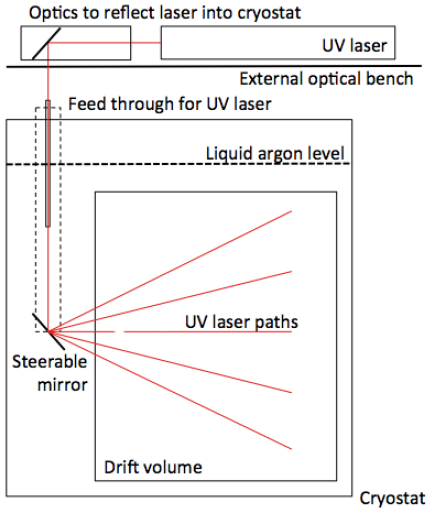
\includegraphics[width=0.45\linewidth]{uB_laser_schematic}
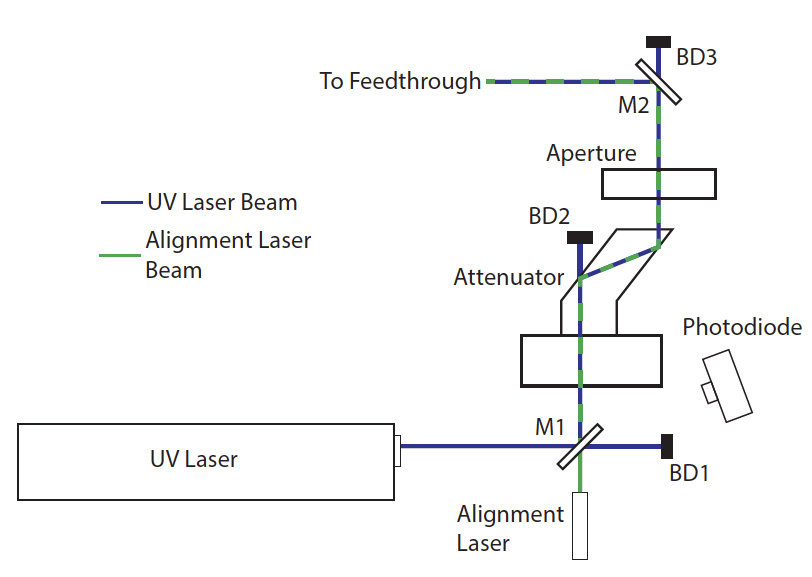
\includegraphics[width=0.5\linewidth]{uB_laser_box}
\end{dunefigure}



For each of those \num{20} ports, a laser module can be schematically represented by Figure~\ref{fig:uB_laser_schematic} (Left), and consists of the following elements:
\begin{itemize}
    \item A laser box (see Figure \ref{fig:uB_laser_schematic}; Right) that provides
    \begin{itemize}
        \item An attenuator and a collimator to control the intensity and size of the beam;
        \item A photodiode that gives a TPC-independent trigger signal;
        \item A low-power red laser, aligned with the UV one, to facilitate alignment operations;
        \item A Faraday cage to shield the surrounding electronics from the accompanying EM pulse.
    \end{itemize}
    \item A feedthrough (see Figure \ref{fig:uB_laser_ft}; Left) into the cryostat that provides:
    \begin{itemize}
        \item The optical coupling that allows the UV light to pass through into the cryostat directly into the liquid phase, avoiding distortions due to the gas-liquid interface and the gas itself;
        \item A rotational coupling that allows the whole structure to rotate while maintaining the cryostat seal;
        \item A periscope structure (see Figure~\ref{fig:uB_laser_ft}; Right) mounted under the rotating coupling that supports a mirror within the \dword{lar};
        \item The additional theta rotation of the mirror accomplished by a precision mechanism coupled to an external linear actuator;
        \item Both the rotation and linear movements of the steering mechanism read out by precision encoders.
    \end{itemize}
    
\end{itemize}


\begin{dunefigure}[\dword{microboone} laser calibration system drawings]{fig:uB_laser_ft}
{CAD drawings of the \dword{microboone} laser calibration system~\cite{microboone}. Left: calibration port feedthrough. Right: laser beam periscope. %Both figures from~\cite{microboone}.
}
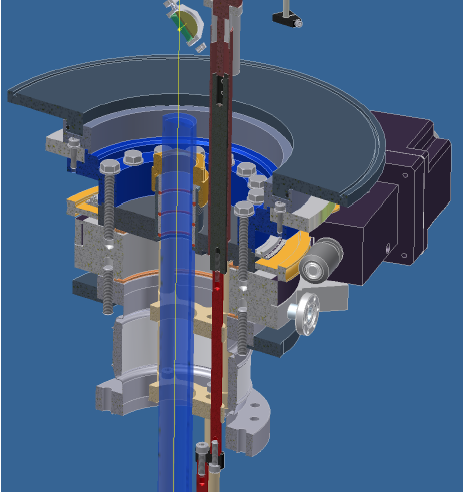
\includegraphics[width=0.49\linewidth]{uB_laser_ft}
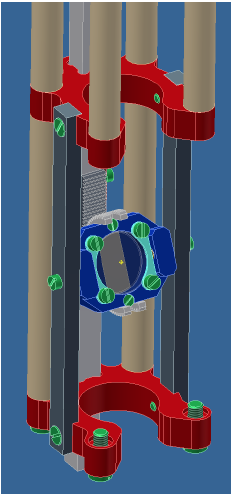
\includegraphics[width=0.248\linewidth]{uB_laser_periscope}
\end{dunefigure}


In the case of the lasers in the end-wall ports, the beams enter the \dword{fc} laterally, while in the case of the lasers in the ports over the TPC, the beams enter the TPC from the top. In both cases, the laser beam can enter the \dword{fc} only through the gaps between the \dword{fc} electrodes. These gaps are \SI{1.4}{\cm} wide and the electrodes themselves are \SI{4.6}{\cm} wide, so it's clear that the shadowed regions are very significant. Section~\ref{sec:sp-calib-laser-alter} describes the alternative designs currently being developed for the laser system. In one of the alternative designs, the top \dword{fc} is modified as to allow small openings for the bottom of the periscope to penetrate %within 
the \dword{fc} (not the ground plane), significantly increasing coverage.

For the six most central ports, the distance between them is small enough that we can consider having the same laser box serving two feedthroughs, in order to reduce the costs associated with the laser and its optics.

%a \SI{266}{\nano\m} laser would be mounted on the top of the cryostat, and service two adjacent feedthroughs. A steerable head and fiber interface would be mounted in the feedthrough, which is coated in a insulator. Two options are under investigation: (1) the \dword{fc} (but not the \dword{gp}) is penetrated, and (2) the \dword{fc} is not penetrated. In the former case, the \dword{fc} penetration has been shown to create a small distortion to the E-field, for the benefit of full volume E-field mapping. When the \dword{fc} is not penetrated, the laser shines through the \dword{fc} tubes, producing some regions that are not mappable by the laser. Unlike the ports that are inwards of the cryostat, the lasers through penetrations that are outside the \dword{fc} on the far east and west side of the cryostat will not penetrate the field cage. The photo-electron system would include a fiber and no steering; the necessity of penetrating the \dword{fc} is unlikely but has not been assessed yet.

A scan of the full detector using \SI{1}{L} volume elements would require a number of tracks on the order of \num{8e5}, 
%would 
and can take about three days. It is expected that shorter runs could be done to investigate specific regions. The sampling granularity, and therefore the amount of data taken, is dependent on \dword{daq} requirements. In fact, even to be able to record the desired \num{8e5} tracks, a dedicated data reduction algorithm will have to be devised, so that only a drift window of about \SI{100}{\micro\s}
of data is recorded, and the position of that window depends on the beam position and direction and which wires are being read out. More details on this are given in section~\ref{sec:sp-calib-daqreq}.

%The direct ionizing laser system may also be used to create \phel{}s from the cathode, even under low power operation.

%% JM %% end % from early IDR version




%%%%%%%%%%%%%%%
%\subsubsubsection{Possible Measurements}
\subsubsection{Measurement Program}
\label{sec:sp-calib-sys-las-ion-meas}


The method for \efield measurement is based on the measurement of position displacements. The laser produces straight tracks in a known position and deviations from that seen in reconstructed tracks are attributed to \efield distortions. Therefore the precision with which the \efield distortions can be measured depends on the precision with which we can know the laser track position and the TPC position reconstruction precision.
The TPC precision in the $y$, $z$ coordinates is given primarily by the wire spacings of \uvpitch and \xgpitch. It is slightly better than that (about \SI{2}{\milli\m}) on the $x$ coordinate, determined by the \fepeaktime peaking time of the front-end electronics.
Given infinite laser positioning accuracy, the smallest measurable \efield distortions would be those that cause displacements of this magnitude --- \SI{2}{\milli\m} in $x$ and \SI{5}{\milli\m} in $y$, $z$. The precision on the drift velocity distortions depends on the size of the spatial region where they are present. For distortions present in regions of \SI{0.5}{\m} and larger, drift velocity distortions can therefore be measured with an accuracy of \SI{1}{\%} in $y$, $z$ and \num{0.4}\% in $x$. In $y$, $z$, \SI{1}{\%} precision on drift velocity distortions translates to a \SI{1}{\%} precision on the transverse field distortions. Along $x$, one must consider that, at \spmaxfield, a \SI{1}{\%} change in \efield leads to a \SI{0.375}{\%} change in drift velocity. Therefore finally, this means that the smallest measurable distortions given the TPC design (wire pitch, timing precision) are of \SI{1}{\%} in \efield if they are present in regions of \SI{0.5}{\m} and larger (smaller field distortions could be in principle be measurable if they are present over larger regions, so that their effect accumulates over the drift path).
On one side, this gives us an ultimate limit to the \efield precision achievable with the laser system, but on the other side, since these TPC precision considerations apply to physics events also, it tells us that an \efield precision much better than \SI{1}{\%} should not have an impact on physics.

In principle, if we were confident about the field in one detector region and would like to probe another, we could use tracks that cross both regions and use the TPC measurements in the ''good'' region as the ``true'' track direction, without needing the hardware information on the mirror angles, etc. But in a general case, the TPC precision is only one of the components of the laser measurement precision, the other being the mechanical beam positioning accuracy. The goal of the mechanical design of the system is to achieve a precision close to that of the TPC measurements, so that no single factor is dominant in the overall systematics. The starting point of the laser beams is given by the position of the mirror in the periscope, that is known from construction drawings and cool down calculations. Warm surveys might be necessary. The angle of the beam is given by the angles ($\theta$, $\phi$) of the mirror, that are set by the periscope motors and read-out by the encoders. 
Reference~\cite{bib:chen2018} quotes a mechanical precision of \SI{0.05}{\mrad} for the \dword{microboone} system, for both angles. At \SI{10}{\m}, the maximum distance in \dword{microboone}, 
%that's \SI{0.5}{\milli\m}.
which results in \SI{0.5}{\milli\m} precision. In DUNE, we 
%count on having 
expect \SI{20}{\m} long beams, so the precision is \SI{1}{\milli\m} 
%at that distance, if we equal 
using the precision of the \dword{microboone} system. The beam itself is wider than that. In fact, with a \SI{0.5}{\mrad} divergence, we expect the beam to be \SI{1}{\cm} wide at \SI{20}{\m}. The profile is Gaussian, so the centroid of the charge creation should be more accurate. During cool down, there can be shifts that need to be measured and corrected for, so we aim to have a system that can measure the beam position in a few positions, at least one per drift volume and laser beam. Our goal is to provide the position of the beam to an accuracy of \SI{5}{\milli\m} with positioning systems located at about \SI{10}{\m} from the beam origin. A laser positioning system is described in the next section.

 
 %% JM %% discuss how to get the \efield from the measurements even if the absolute knowledge of the laser track is not perfect.
 % - need for crossing tracks
 % - use positioning system
 % - do relative measurements between tracks close by. actual advantage of the alternative system: many parallel tracks at different x
 
 % also, estimate time needed and discuss idea of having the photo-laser for a quick/rough monitoring, and the ionization laser as a detailed probe of regions identified as possibly problematic.


%The remaining studies for the laser systems to be done prior to the \dword{tdr} are: 
%\begin{itemize}
%\item Determine a nominal design for photoelectric thin metal surfaces on the cathode. A survey in cold conditions is not possible for the \single system, and the photoelectric system could provide both known positions in the detector and information complementary to a survey or cosmic data.
%\item For the \dual system, quantify the additional benefit of a photoejection system since it will be possible to survey the \dwords{crp} externally under cold conditions.
%\item  Determine whether the known classes of possible \efield distortions warrant a mechanical penetration of the \dword{fc} (versus reduced sampling from projecting laser light inward between \dword{fc} elements) and further understand sensitivity of the laser to realistic \efield distortions. 
%\item Continue to study the range of possible \efield distortions in order to further refine the estimation of overall variation of the \efield  in the \dword{detmodule}. 
%\end{itemize}
%\begin{itemize}
%\item Determine  a nominal design for photoelectric targets on the cathode, and whether  such targets would provide sufficient survey-like information.
%\item Determine if the known classes of possible \efield distortions require penetration of the \dword{fc} (versus reduced sampling from shining between the field cage). 
%\item Further understand limitations on laser location precision, practical range of propagation due to optics design and Rayleigh scattering. \fixme{KM: Is this too vague to be helpful or sets us up for failure? What specifically will be studied?}
%\item Continue to quantify the range of possible \efield distortions in the DUNE FD to further refine the estimation of overall variation of \efield (both locally and globally) in the detector.
%\end{itemize}

%\fixme{}

